% !TeX spellcheck = es_ES
%%%%%%%%%%%%%%%%%%%%%%%%%%%%%%%%%%%%%%%%%%%%%%%%%%
% Plantilla presentación Beamer no oficial - Universidad Nacional de Colombia
%%%%%%%%%%%%%%%%%%%%%%%%%%%%%%%%%%%%%%%%%%%%%%%%%%
%------------------
% LICENCE
%------------------
% Copyright (c) 2023 by Fabio Calderón
%
% This work is licensed under the Creative Commons Attribution 4.0 International License. (CC BY-NC-SA 4.0)
%
% To view a copy of this license, visit ``http://creativecommons.org/licenses/by-nc-sa/4.0/'' or send a letter to Creative Commons, PO Box 1866, Mountain View, CA 94042, USA.
%------------------
% IMPORTANT: Read the instructions (in comment format) in each file of this template.
%
% This template has been developed following the identity guidelines of the Universidad Nacional de Colombia (https://identidad.unal.edu.co/).
%------------------
% REQUIREMENTS
%------------------
% The beginning of the document with "\documentclass[aspectratio=169,usenames,dvipsnames]{beamer}" is mandatory since the template has been developed for the 16:9 aspect ratio and requires the "xcolor" and "tikz" packages.
%------------------
% CREDITS
%------------------
% This template is an adaptation of the public file "University of Udine Unofficial Beamer Theme" by Marco Basaldella (Creative Commons CC BY 4.0). Available at: https://www.overleaf.com/latex/templates/university-of-udine-unofficial-beamer-theme/zndkgxrjsdzt.
%
% Elements have also been taken from the "Leiden University Beamer Theme" by J.P. van Leenen (LaTeX Project Public License 1.3c). Available at: https://www.overleaf.com/latex/templates/leiden-university-beamer-theme/ryfcpypnvzhr.
%
% Image credits:
% - Cover: "Skyscrapers in Bogota's downtown" by Mayor's Office of Bogota. https://commons.wikimedia.org/wiki/File:Bogota_Skyline.jpg. CC BY-SA 4.0.
% - framepic background: "Biblioteca Ernesto Guhl, Ciudad Universitaria, Universidad Nacional de Colombia" by Rubashkyn. https://commons.wikimedia.org/wiki/File:Biblioteca_Ernesto_Guhl,_Universidad_Nacional,_Bogot%C3%A1.JPG. GFDL.
% - UNAL Logos: identidad.unal.edu.co.
%------------------
% ABOUT THE AUTHOR
%------------------
% Developed by Fabio Calderón in his fourth and final year of the Doctorate in Mathematical Sciences at the National University of Colombia.
% Suggestions/Comments: facalderonm@unal.edu.co
%------------------
% TODO
%------------------
% - Fix warnings of overfull at frames with title.
%%%%%%%%%%%%%%%%%%%%%%%%%%%%%%%%%%%%%%%%%%%%%%%%%%
%------------------
% DOCUMENT TYPE
%------------------
\documentclass[aspectratio=169,10pt,usenames,dvipsnames,spanish]{beamer}
%\documentclass[aspectratio=169,usenames,dvipsnames,spanish]{beamer}
% Replace "spanish" for "english" or any other language.
%%%%%%%%%%%%%%%%%%%%%%%%%%%%%%%%%%%%%%%%%%%%%%%%%%
%------------------
% DOCUMENT THEME
%------------------
\usetheme{UNAL}
%%%%%%%%%%%%%%%%%%%%%%%%%%%%%%%%%%%%%%%%%%%%%%%%%%
%------------------
% PACKAGES
%------------------
\usepackage{graphics,graphicx} % To insert graphs. They must be in the same folder than the .TEX file.
\usepackage{amsthm, amssymb, amsfonts, latexsym, mathtools,thmtools,bbm} % Enviroments and several math symbols.
\usepackage{ragged2e} % Justifies text.
\usepackage{tikzsymbols} % Emojis.
\usepackage{comment} % To comment huge portions of text.
\usepackage{multicol} % For multiple columns of text or listings.
\usepackage{verbatim} % For code-style text.
% Add any additional packages that are needed here.
\usepackage{mathrsfs}


\usepackage{fontspec}   %yesid
\setmainfont{Ancizar Sans}   %yesid
\setsansfont{Ancizar Sans}   %yesid



\usepackage[backend=biber,style=authoryear]{biblatex}   %yesid
\addbibresource{references.bib}   %yesid
%\bibliographystyle{plain} %yesid

\newcommand{\ve}[1]{\mathbf{#1}}    %Creado por Yesid
\newcommand{\vg}[1]{\boldsymbol{#1}}   %Creado por Yesid
\newcommand{\ite}{\hat{\imath}} %Creado por Yesid
\newcommand{\jte}{\hat{\jmath}} %Creado por Yesid
\newcommand{\kte}{\hat{k}} %Creado por Yesid


\usepackage{listings}
\usepackage{xcolor}

\lstset{
  basicstyle=\ttfamily\small,
  keywordstyle=\color{blue},
  commentstyle=\color{green!60!black},
  stringstyle=\color{red},
  showstringspaces=false,
  breaklines=true,
  frame=single
}


%%%%%%%%%%%%%%%%%%%%%%%%%%%%%%%%%%%%%%%%%%%%%%%%%%
%------------------
% INFO
%------------------
\title[Plantilla Beamer]{Movimiento de una partícula con espín en relatividad general: analogías y diferencias con el electromagnetismo}
%\subtitle{Para la Universidad Nacional de Colombia}
\author[Autor]{Yesid Fernando Guerrero Guio}
\institute{Departamento de física}
\date{\today}
\rotulo{Director}
\director{Juan Manuel Tejeiro Sarmiento}
\institutedos{Observatorio astronómico nacional}
% IMPORTANT: If any of the parameters are too long for the cover or require multiple lines (e.g., extensive title), their arrangement can be modified in the "beamerinnerthemeUNAL.sty" file.
%%%%%%%%%%%%%%%%%%%%%%%%%%%%%%%%%%%%%%%%%%%%%%%%%%
%%%%%%%%%%%%%%%%%%%%%%%%%%%%%%%%%%%%%%%%%%%%%%%%%%
%%%%%%%%%%%%%%%%%%%%%%%%%%%%%%%%%%%%%%%%%%%%%%%%%%
\begin{document}
\justifying % This command justifies all text OUTSIDE of boxes/environments. To also justify text inside boxes/environments, you should use this same command within the box/environment, just right before the text.
%------------------
% COVER
%------------------
\begin{frame}
    \titlepage 
    % The background image, its opacity, and position can be modified in the file "beamerinnerthemeUNAL.sty".
\end{frame}
%------------------
% TAABLE OF CONTENTS
%------------------
\begin{frame}{Contenidos}
    \tableofcontents
\end{frame}

%%%%%%%%%%%%%%%%%%%%%%%%%%%%%%%%%%%%%%%%%%%%
%%%%%%%%%%%%%%%% INTRODUCCION %%%%%%%%%%%%%%%%%%
%%%%%%%%%%%%%%%%%%%%%%%%%%%%%%%%%%%%%%%%%%%%

\section{Introducción}

\begin{frame}
\frametitle{Movimiento en espacio-tiempo curvo}

\begin{columns}

% -------- COLUMNA TEXTO --------
\begin{column}{0.55\textwidth}
\textbf{Geodésicas}
La trayectoria de una partícula sin estructura interna:
\begin{equation}
\ddot{x}^\mu+\Gamma^\mu_{\nu\rho}\dot{x}^\nu\dot{x}^\rho=0
\end{equation}

\vspace{0.3cm}

\textbf{Partículas con espín}

En la aproximación polo-dipolo ( Ecuaciones de Mathisson–Papapetrou–Dixon), el movimiento difiere de las geodésicas:

\begin{equation}\label{EcuMomento}
\frac{Dp^\mu}{d\tau}=- \frac{1}{2} R^\mu{}_{\nu\kappa\lambda}u^\nu S^{\kappa\lambda}
\end{equation}

\begin{equation}\label{EcuEspín}
\frac{DS^{\mu\nu}}{d\tau}= p^\mu u^\nu- u^\mu p^\nu
\end{equation}

\end{column}

% -------- COLUMNA IMAGEN --------
\begin{column}{0.4\textwidth}
\centering
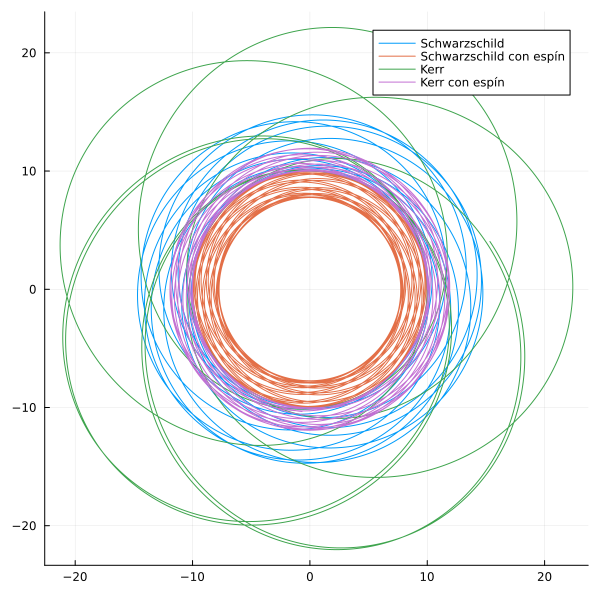
\includegraphics[width=\linewidth]{graphics/trayectorias}

\vspace{0.2cm}

{\scriptsize Trayectorias de partículas con y sin espín en las métricas de Schwarzschild y Kerr.\\
Cond. in: $r_0=10$, $\theta_0=\pi/2$, $\phi_0=0$, $v_0=0$, $a=s=0.9$.}
\end{column}

\end{columns}

\end{frame}


%%%%%%%%%%%%%%%%%%%%%%%%%%%%%%%%%%%%%%%%%%%%
%%%%%%%%%%%%%%%% INTRODUCCION 2 %%%%%%%%%%%%%%%%%
%%%%%%%%%%%%%%%%%%%%%%%%%%%%%%%%%%%%%%%%%%%%

\begin{frame}
\frametitle{Cuadrimomento de una partícula con espín}

A partir de la contracción con $u_\nu$ y usando $u^\mu u_\mu=-c^2$, se obtiene:

\begin{equation}\label{Momentoespin}
    p^\mu = m u^\mu - \frac{u_\nu}{c^2} \frac{D S^{\mu\nu}}{d\tau}
\end{equation}

\vspace{0.4cm}
es posible definir una masa $\mu$ y una velocidad dinámica $v^\mu$ tal que cumpla $p^\mu=\mu v^\mu$, donde $v^\mu v_\mu=-c^2$ y por lo tanto \cite{Gerakopoulos2014,Knickmann2015,Ehlers1979}.
\vspace{0.4cm}
\begin{columns}

\column{0.5\textwidth}
\textbf{Masa cinemática}
\begin{equation*}
    m = -\frac{p^\nu u_\nu}{c^2}
\end{equation*}


\column{0.5\textwidth}
\textbf{Masa dinámica}
\begin{equation*}
    \mu^2 = -\frac{p^\mu p_\mu}{c^2}
\end{equation*}
\end{columns}


Con el fín de cerrar el sistema es necesario definir unas condiciones suplementarias de espín (SSC) que además también establecen una línea de mundo en la partícula y permiten encontrar una relación entre $u^\mu$ y $p^\mu$.
\end{frame}



%%%%%%%%%%%%%%%%%%%%%%%%%%%%%%%%%%%%%%%%%%%%
%%%%%%%%%%%%%%%% INTRODUCCION 3 %%%%%%%%%%%%%%%%%
%%%%%%%%%%%%%%%%%%%%%%%%%%%%%%%%%%%%%%%%%%%%



\begin{frame}
\frametitle{Comparación de condiciones suplementarias de espín}

\begin{columns}[t]

%------------------ Columna 1 ------------------
\begin{column}{0.59\textwidth}
\textbf{Tulczyjew (TSSC)}

\vspace{0.3cm}

\begin{equation}
S^{\mu\nu}p_\nu = 0
\end{equation}

\vspace{0.3cm}


\begin{equation}
u^\mu = N \left(v^\mu + \frac{1}{2c^2\mu^2\Delta_s}
R_{\nu\sigma\kappa\lambda}S^{\mu\nu}S^{\kappa\lambda}v^\sigma \right)
\end{equation}

\vspace{0.3cm}

\begin{equation}
\Delta_s = 1 + \frac{1}{4\mu^2 c^2}
R_{\sigma\delta\kappa\lambda}S^{\sigma\delta}S^{\kappa\lambda}
\end{equation}

\vspace{0.3cm}

\begin{equation}
N = \frac{c}{\left[c^2 - \frac{1}{4\mu^4 \Delta_s^2 c^4}
R_{\nu\sigma\kappa\lambda}R^{\alpha\beta\gamma\delta}
S^{\mu\nu}S^{\kappa\lambda}S_{\mu\alpha}S_{\gamma\delta}
v^\sigma v_\beta \right]^{1/2}}
\end{equation}

\end{column}

%------------------ Columna 2 ------------------
\begin{column}{0.45\textwidth}
\textbf{Mathisson-Pirani (MP SSC)}

\vspace{0.3cm}

\begin{equation}
S^{\mu\nu}u_\nu = 0
\end{equation}

\vspace{0.3cm}

\begin{equation}
u^\mu = v^\mu
\end{equation}

\vspace{0.3cm}

\begin{equation}
u^\mu = \frac{1}{m}\left(p^\mu + 
\frac{S^{\mu\nu}S_{\nu\beta}p^\beta}{S^2}\right)
\end{equation}

\end{column}

\end{columns}

\end{frame}

%%%%%%%%%%%%%%%%%%%%%%%%%%%%%%%%%%%%%%%%%%%%
%%%%%%%%%%%%%%%% INTRODUCCION 3 %%%%%%%%%%%%%%%%%
%%%%%%%%%%%%%%%%%%%%%%%%%%%%%%%%%%%%%%%%%%%%

\begin{frame}
\frametitle{Aproximación espín débil}
En el régimen en el que los términos cuadráticos en el espín puedan despreciarse, las ecuaciones de la SSC se reducen a:

\begin{equation}\label{aproximaciones}
	\Delta_s \approx 1 \hspace{0.5cm} N \approx 1 \hspace{0.5cm} u^\mu \approx p^\mu
\end{equation}

por lo tanto, la masa cinemática es aproximadamente igual a la masa dinámica $\mu \approx m$, y
\begin{equation}\label{Condiciones TSSC y PSSC}
	S^{\mu\nu}p_\nu=S^{\mu\nu}\mu v_\nu=0   \Longrightarrow   S^{\mu\nu} u_\nu \approx 0
\end{equation}
es decir, en el límite de espín débil, las condiciones de Tulczyjew y Pirani son aproximadamente las mismas. La ecuación \ref{Momentoespin} se reduce a $p^\mu \approx mu^\mu$, y reemplazando en (\ref{EcuMomento}) se obtiene la fuerza espín-curvatura de Mathisson-Papapetrou:

\begin{equation}\label{FuerzaMPD}
	f^\mu=m \frac{D u^\mu}{d \tau}=- \frac{1}{2} R^\mu{}_{\nu\kappa\lambda}u^\nu S^{\kappa\lambda}
\end{equation}
\end{frame}
%%%%%%%%%%%%%%%%%%%%%%%%%%%%%%%%%%%%%%%%%%%%
%%%%%%%%%%%%%%%%% FUNDAMENTOS %%%%%%%%%%%%%%%%%%
%%%%%%%%%%%%%%%%%%%%%%%%%%%%%%%%%%%%%%%%%%%%
\section{Fundamentos}
\begin{frame}
\frametitle{Métrica de Kerr}
En 1963, Roy Kerr propuso la solución en el vacío a las ecuaciones de campo de Einstein
, de una fuente en rotación con simetría axial \cite{Kerr1963}. La métrica de Kerr depende de dos cantidades físicas: la masa $M$ y la rotación descrita por el parámetro $a$. La solución es estacionaria y axialmente simétrica, esto se evidencia en el elemento de línea que no depende de $t$ y $\phi$:
\begin{multline} \label{Metrica_Kerr}
ds^2=-c^2\left(1-\frac{2G_NMr}{c^2\rho^2}\right)dt^2+\frac{\rho^2}{\Delta}\, dr^2+\rho^2 \,d\theta^2\\+\left(r^2+a^2+\frac{2G_NMa^2r \sin^2 \theta}{c^2 \rho^2}\right)\sin^2 \theta \,d\phi^2-\frac{4G_NMar}{c^2\rho^2}\sin^2\theta\, c\,dt\, d\phi
\end{multline}
donde
\begin{align} \label{eq1}
\rho^2 &= r^2+a^2 \cos^2\theta \\ 
\Delta&=r^2-\frac{2G_NMr}{c^2}+a^2
\end{align}


con $a=J/(Mc)$, siendo $a$ el momento angular por unidad de masa del objeto masivo.
\end{frame}





\section{Gravitoelectromagnetismo}
%%%%%%%%%%%%%%%%%%%%%%%%%%%%%%%%%%%
%%%%%% GEM basado en la teoría linealizada %%%%%%%%%
%%%%%%%%%%%%%%%%%%%%%%%%%%%%%%%%%%%
\subsection{Basado en la teoría linealizada}
\begin{frame}
\frametitle{GEM basado en la teoría linealizada}
%\begin{frame}{\color{black}\textbf{Gravitomagnetismo basado en la linealización de las ecuaciones de Einstein}}
En la aproximación de campo débil $g_{\mu \nu}=\eta_{\mu \nu}+h_{\mu \nu}$, donde $|h_{\mu \nu}|\ll1$ \parencite{Bambi2018}. Asumiendo $g_{\mu \nu, t}=0$ y despreciando los términos $O(h^2)$, entonces los símbolos de Christoffel son:
\begin{equation}\label{SimbolosChristoffel}
    \Gamma^\kappa_{\nu \sigma}=\frac{1}{2}\eta^{\kappa\lambda}(h_{\lambda\sigma,\nu}+h_{\nu\lambda,\sigma}-h_{\nu\sigma,\lambda})
\end{equation}

 \begin{equation}\label{TensorRicci_Esca_Linealizadas}
        R_{\mu\nu}=\frac{1}{2}\eta^{\lambda\sigma}(h_{\sigma\nu,\mu\lambda}-h_{\mu\nu,\sigma\lambda}-h_{\sigma\lambda,\mu\nu}+h_{\mu\lambda,\sigma\nu}), \hspace{1cm} R=h^{\mu\lambda},_{\mu\lambda}-h_{\mu}{}^\mu,_\lambda{}^{\lambda}
    \end{equation}
    
Reemplazando \ref{TensorRicci_Esca_Linealizadas} en las ecuaciones de campo, y aplicando $\bar{h}_{\mu\nu}=h_{\mu\nu}-1/2\,n_{\mu\nu}\,h$ obtenemos :
    \begin{equation}\label{EqEinsteinLinealizadash}
        -\bar{h}_{\mu\nu,\lambda}{ }^{\lambda}-\eta_{\mu\nu}\bar{h}_{\sigma\lambda}{}^{,\sigma\lambda}+\bar{h}_{\mu\lambda,\nu}{}^{\lambda}+\bar{h}_{\nu\lambda,\mu}{}^{\lambda}=\frac{16\pi}{c^4}G T_{\mu\nu} \hspace{0.4cm} \Rightarrow \hspace{0.4cm}         -\bar{h}_{\mu\nu,\lambda}{}^{\lambda}=\frac{16 \pi G T_{\mu\nu}}{c^4}
    \end{equation}
    
  imponiendo el Gauge de Lorentz $\bar{h}^{\mu\alpha}{}_{,\alpha}=0$ (La transformación infinitesimal $h_{{\mu'}{\nu'}}^{nuevo}=h_{\mu\nu}^{ant}-\xi_{\mu,\nu}-\xi_{\nu,\mu}$ dejan invariante el tensor de Riemann) \parencite{Misner1973}
\end{frame}

%%%%%%%%%%%%%%%%%%%%%%%%%%%%%%%%%%%
%%%%%%%Solución a las ecuaciones linealizadas%%%%%%%%
%%%%%%%%%%%%%%%%%%%%%%%%%%%%%%%%%%%

\begin{frame}
\frametitle{Solución a las ecuaciones linealizadas}
    En $\gamma\approx1$, $u^\mu\approx(c,\ve{u})$, y $T^{\mu\nu}\equiv\rho u^\mu u^\nu$, entonces $T^{tt}\equiv\rho c^2$, $T^{ij}\equiv\rho u^i u^j$ y $T^{ti}\equiv cj^i$. Definimos los potenciales $\Phi$ y $A^i$ \parencite{SJ2020, Mashhoon1999}:
\begin{equation}\label{potencialesGEM}
    \Phi(\mathbf{r})\equiv -G\int \frac{\rho(\mathbf{r'})}{|\mathbf{r}-\mathbf{r'}|}d^3r' \hspace{2cm} A^i(\mathbf{r})\equiv -\frac{2G}{c^2}\int \frac{j^i(\mathbf{r'})}{|\mathbf{r}-\mathbf{r'}|}d^3r'
\end{equation}

La métrica se puede escribir como:
\begin{equation}\label{ElementoLinea}
    ds^2=-c^2\left(1+\frac{2\Phi}{c^2}\right)dt^2+\left(1-\frac{2\Phi}{c^2}\right)\delta_{ij}dx^idx^j+4\mathbf{A}\cdot d\mathbf{x}dt
\end{equation}

La métrica de Kerr para un cuerpo de rotación baja y campo débil, es decir, $a \ll1$ y $2GM/(c^2r) \ll 1$:
\begin{multline}
ds^2=-c^2\left(1-\frac{2G_NM}{c^2r}\right)dt^2
+\left(1+\frac{2G_NM}{c^2r}\right)\, dr^2 \\ 
+r^2 \,d\theta^2+r^2\sin^2 \theta \,d\phi^2
+\text{\fcolorbox{red}{white}{$-\frac{4G_NJ}{c^2r}\sin^2\theta$}}\, dt\, d\phi
\end{multline}
\end{frame}



%%%%%%%%%%%%%%%%%%%%%%%%%%%%%%%%%%%
%%%%%%%% Ecuaciones de campo linealizadas %%%%%%%%
%%%%%%%%%%%%%%%%%%%%%%%%%%%%%%%%%%%

\begin{frame}
\frametitle{Ecuaciones de campo linealizadas}
De manera similar al electromagnetismo podemos definir los campos gravitoelectromagnéticos como:
\begin{equation}\label{CamposGEM}
    \mathbf{E}\equiv-\nabla \Phi-\frac{\partial}{\partial t}\left(\frac{1}{2}\mathbf{A}\right) \hspace{2cm} \mathbf{B}\equiv\nabla \times\mathbf{A}
\end{equation}

Las ecuaciones de campo de Maxwell para el gravitomagnetismo:


\begin{equation}\label{GaussGE_GM}
    \mathbf{\nabla}\cdot \mathbf{E}=-4\pi G \rho \hspace{1cm} \hspace{1cm} \nabla \cdot\left(\frac{1}{2} \mathbf{B}\right)=0
\end{equation}

\begin{equation}\label{LeyFaraday GEM1}
    \nabla \times \mathbf{E}=-\frac{\partial}{\partial t} \left(\frac{1}{2}\mathbf{B}\right) \hspace{1cm}     \nabla\times\left(\frac{1}{2}\mathbf{B}\right)=\frac{1}{c^2}\frac{\partial \mathbf{E}}{\partial t}-\frac{4\pi G}{c^2} \mathbf{j}
\end{equation}

La fuerza de Lorentz del gravitoelectromagnetismo a partir de la componente espacial de la ecuación geodésica:

\begin{equation}\label{LorenztGEM1}
    \mathbf{F}=m(\mathbf{E}+2\mathbf{v}\times\mathbf{B})
\end{equation}

\end{frame}

%%%%%%%%%%%%%%%%%%%%%%%%%%%%%%%%%%%
%%%%%%%%%%% GEM fuerzas inerciales %%%%%%%%%%%
%%%%%%%%%%%%%%%%%%%%%%%%%%%%%%%%%%%
\subsection{Basado en fuerzas inerciales}
\begin{frame}
\frametitle{GEM basado en fuerzas inerciales}

Un marco de referencia propio de un observador acelerado es definido en \parencite{Misner1973} de la siguiente manera: Sea $\tau$ el tiempo propio medido por un observador acelerado que se mueve en una linea de mundo $\mathcal{P}=\mathcal{P}(\tau)$, donde la base tetradica ortonormal es definido como
\begin{equation}\label{Aecu: etetrada}
	\hat{e}_{0}(\tau)=u_{N}(\tau) \hspace{1cm} \hat{e}_{\alpha}\cdot \hat{e}_{\beta}=\hat{\eta}_{\alpha\beta}
\end{equation}

con $u_{N}(\tau)=u(\tau)/c$ es la cuadrivelocidad normalizada del observador \parencite{Hobson2015}, cuya evolución a lo largo de la linea de mundo esta dado por

\begin{equation}\label{Aecu:evolucion tetrada}
	\nabla_{\hat{u}}\hat{e}_{\beta}=\hat{\Omega}^{\alpha}{}_{\beta}\hat{e}_{\alpha}; \hspace{0.5cm} \Omega^{\alpha\beta}=\frac{2}{c^2}u^{[\alpha}a^{\beta]}+\frac{1}{c}\tilde{\epsilon}^{\;\alpha\beta}{}_{\nu\mu}\Omega^\mu u^\nu
\end{equation}

donde $\Omega^{\mu\nu}$ es el generador de transformación infinitesimal de Lorentz \parencite{Misner1973}. El término $(2/c^2)u^{[\alpha}a^{\beta]}$ es el transporte Fermi-Walker, y $\vg{\Omega}$ es la velocidad angular de rotación de la triada espacial $\hat{e}_{i}$ relativo a la triada transportada Fermi-Walker. Las componentes espaciales del generador estan dadas por $\hat{\Omega}_{ij}=\hat{\epsilon}_{ikj}\hat{\Omega}^{k}$,  \parencite{Costa2014}. Si $\Omega^{\mu}=0$ se recupera el tranporte Fermi-Walker, si además $a^{\mu}=0$ se recupera el transporte paralelo.

\end{frame}

%%%%%%%%%%%%%%%%%%%%%%%%%%%%%%%%%%%
%%%%%% Congruencia de observadores acelerados %%%%%%
%%%%%%%%%%%%%%%%%%%%%%%%%%%%%%%%%%%

\begin{frame}
\frametitle{Congruencia de observadores y componentes de la conexión}
\begin{columns}[t] % 't' para alinear arriba ambas columnas
    %-----------------------------------
    % Columna izquierda: texto
    %-----------------------------------
    \begin{column}{0.58\textwidth}
        El espacio-tiempo es cubierto por un conjunto de curvas temporales 
        $\mathcal{P}_{\mathsf{x}} (\tau)$, donde $\mathsf{x}$ es el número de la curva, $\tau$ el tiempo propio del observador; y el vector tangente  
        es $u^\mu=\partial x^\mu/\partial \tau$, y el \textit{vector de desviación} es $\mathcal{X}^\mu=\partial x^\mu/\partial \mathsf{x}$.             La proyección espacial de la derivada covariante de $u^{\alpha}$:
        \begin{equation}
            K^{\alpha\beta}\equiv (h^u)^{\alpha}{}_{\lambda}(h^u)^{\beta}{}_{\tau}\nabla^{\tau}u^{\lambda}
            =\nabla^{\beta}u^{\alpha}+\frac{1}{c^2}u^{\beta}a^{\alpha} 
        \end{equation}
        El cual se puede descomponer en su traza $\theta$ (expansión), 
        su parte simétrica libre de traza $\sigma_{\alpha\beta}$ (cizalladura), 
        y la parte antisimétrica $\omega_{\alpha\beta}$ (vorticidad):
        \begin{align}\label{Aecu:descoK}
            K_{\alpha\beta}=K_{(\alpha\beta)}+K_{[\alpha\beta]}=
            \sigma_{\alpha\beta}+\frac{1}{3}\theta h_{\alpha\beta}+\omega_{\alpha\beta}
        \end{align}
    \end{column}

    %-----------------------------------
    % Columna derecha: imagen + ecuaciones
    %-----------------------------------
    \begin{column}{0.38\textwidth}
        \begin{figure}[t]
            \centering
            % reducimos el tamaño un poco
            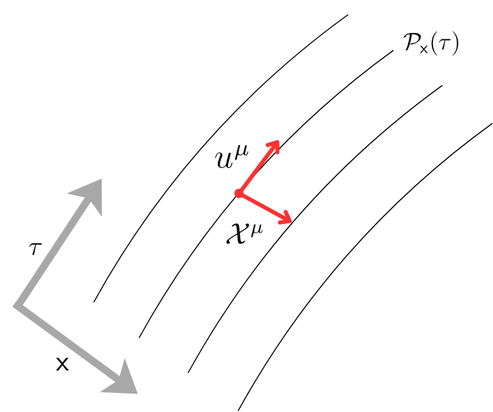
\includegraphics[width=0.85\linewidth]{graphics/CongruenciaObservadores.png}
            \caption{\scriptsize Congruencia de observadores. Imagen generada a partir de \parencite{Carroll2004}.}
            \label{fig:CongruenciaObservadores}
        \end{figure}

 
    \end{column}
\end{columns}
Los componentes de $\hat{\Gamma}^{\mu}_{\nu\sigma}$ en este marco son: 
\begin{equation}\label{Aecu:ComponentesGamma1}
	\hat{\Gamma}^{0}_{00}=0, \hat{\Gamma}^{0}_{0j}=\hat{\Gamma}^{j}_{00}=\frac{1}{c^2}\hat{a}_{j}, \hat{\Gamma}^{j}_{0k}=\frac{1}{c}\hat{\epsilon}^{j}{}_{\mu k}\hat{\Omega}^{\mu}
            =\frac{1}{c}\hat{\Omega}^{j}{}_{k},  \hat{\Gamma}^{i}_{j0}=\hat{\Gamma}^{0}_{ji}=\frac{1}{c}\hat{K}_{ij}, \hat{\Gamma}^{0}_{i0}=0
\end{equation}

\end{frame}

%%%%%%%%%%%%%%%%%%%%%%%%%%%%%%%%%%%
%%%%%%%%%% Desarrollo de la analogía %%%%%%%%%%%
%%%%%%%%%%%%%%%%%%%%%%%%%%%%%%%%%%%

\begin{frame}
\frametitle{Desarrollo de la analogía}
En el marco de referencia de una congruencias de observadores acelerados, la componente espacial de la ecuación geodésica de una partícula de prueba que se mueve en el espacio-tiempo con cuadrivelocidad $U^{\mu}$.
    \begin{align*}
	\nonumber \hat{\nabla}_{\hat{U}}\hat{U}^{\alpha}&=\frac{D\hat{U}^{\alpha}}{d\tau}=    \frac{d\hat{U}^{i}}{d\tau}+ \hat{\Gamma}^{i}_{00} (\hat{U}^{0})^{2} + (\hat{\Gamma}^{i}_{0j} + \hat{\Gamma}^{i}_{j0}) \hat{U}^{0} \hat{U}^{j}+ \hat{\Gamma}^{i}_{jk} \hat{U}^{k} \hat{U}^{j} = 0
\end{align*}
\begin{equation}
	\frac{\tilde{D}\hat{U}^i}{d\tau}=-\frac{\hat{a}^i}{c^2} (\hat{U}^{0})^{2}+\frac{1}{c} [\hat{U}\times (\hat{\Omega}+\hat{\omega})]^i\hat{U}^{0}-\frac{1}{c}\hat{\sigma}^{i}{}_{j}\hat{U}^{0} \hat{U}^{j}-\frac{1}{3c}\theta\delta^i{}_{j}\hat{U}^{0} \hat{U}^{j}
\end{equation}

se define el campo gravitoeléctrico y el campo gravitomagnético como \parencite{Costa2014}:
\begin{equation}\label{CGEM_inerciales}
	\ve{G}\equiv-\ve{a} \hspace{1cm} \ve{H}\equiv\vg{\omega}+\vg{\Omega}
\end{equation}
entonces en forma vectorial:
\begin{equation}\label{FLorentz_inerciales}
	\frac{\tilde{D} \ve{U}}{d\tau}=\frac{\hat{U}^0}{c}\left[\frac{\hat{U}^0}{c} \ve{G}+\ve{U} \times \ve{H}-\hat{\sigma}^{i}{}_{j} \hat{U}^{j} \hat{e}_{i}-\frac{1}{3}\theta\ve{U}\right]
\end{equation}
se asemeja a la ecuación de movimiento para una partícula con masa $m_e$, carga eléctrica $e$ y velocidad $\ve{u}_e$ ubicada en un campo eléctrico $\ve{E}$ y un campo magnético $\ve{B}$ $d\ve{p}/d\tau=e(u^0\ve{E}+\ve{u}_e\times\ve{B})$ \parencite{Misner1973,MunizOliva2002}
\end{frame}

%%%%%%%%%%%%%%%%%%%%%%%%%%%%%%%%%%%
%%%%%%%%% Formalismo de quasi-Maxwell %%%%%%%%%
%%%%%%%%%%%%%%%%%%%%%%%%%%%%%%%%%%%


\begin{frame}
\frametitle{Formalismo de quasi-Maxwell}
Cuando el espacio-tiempo es estacionario, $h^{\alpha}{}_{\mu}h^{\beta}{}_{\nu}\mathscr{L}_u g_{\alpha\beta}=2\sigma_{\mu\nu}+\frac{2}{3}\theta h_{\mu\nu}=2K_{(\mu\nu)}=0$, es decir que $\theta=0$ y $\sigma_{\mu\nu}=0$ \parencite{MunizOliva2002,Natario2007}.
\begin{equation}\label{FLorentz_inerciales_Quasi}
	\frac{\tilde{D} \ve{U}}{d\tau}=\frac{\hat{U}^0}{c}\left[\frac{\hat{U}^0}{c} \ve{G}+\ve{U} \times \ve{H}\right]
\end{equation}
Además haciendo $\hat{\Omega}_{ij}=\hat{\omega}_{ij}=-\frac{1}{2}\epsilon_{ijk}\hat{H}^k$ y $\hat{H}_{ij}=\epsilon_{ijk}\hat{H}^k$ entonces $\hat{K}_{[ij]}=-\epsilon_{ijk}\hat{H}^k/2$

 las componentes del tensor de Riemann son:
\begin{align}
	\label{Ecuacion:R0i0j estacionario} \hat{R}_{0i0j}&=-\frac{1}{c^2}\hat{\tilde{\nabla}}_j\hat{G}_i+\frac{1}{c^4}\hat{G}_j\hat{G}_i-\frac{1}{4c^2}\hat{H}^{m}{}_{j}\hat{H}_{im}\\
	\label{Ecuacion:R0ijk estacionario} \hat{R}_{0ijk}&=-\frac{1}{2c}\hat{\nabla}_k\hat{H}_{ij}+\frac{1}{2c}\hat{\nabla}_j\hat{H}_{ik}-\frac{1}{c^3}\hat{H}_{jk}\hat{G}_i\\
	\label{Ecuacion:Rijkl estacionario} \hat{R}_{ijkl}&=\hat{\tilde{R}}_{ijkl}+\frac{1}{4c^2}\hat{H}_{ik}\hat{H}_{jl}-\frac{1}{4c^2}\hat{H}_{il}\hat{H}_{jk}+\frac{1}{2c^2}\hat{H}_{kl}\hat{H}_{ij}
\end{align}
\end{frame}


%%%%%%%%%%%%%%%%%%%%%%%%%%%%%%%%%%%
%% Ecuaciones de campo en la analogía de fuerzas inerciales %%
%%%%%%%%%%%%%%%%%%%%%%%%%%%%%%%%%%%

\begin{frame}
\frametitle{Ecuaciones de campo en la analogía de fuerzas inerciales}
\begin{center}
\renewcommand{\arraystretch}{1.0} % separa un poco las filas
\setlength{\tabcolsep}{1pt} % espacio entre columnas

\begin{tabular}{p{0.30\textwidth} p{0.60\textwidth}}
\textbf{Electromagnetismo} 
& 
\textbf{Gravitoelectromagnetismo} \\[0.4cm]

$F^{\alpha\beta}{}_{;\beta} = 4\pi J^{\alpha}$ 
& $R_{\mu\nu} = \frac{8\pi G_N}{c^4}\left(T_{\mu\nu} - \tfrac{1}{2}g_{\mu\nu}T^{\alpha}{}_{\alpha}\right)$ \\[0.4cm]

$\tilde{\ve{\nabla}}\cdot\ve{E} =\frac{\rho_c}{\epsilon_0} + \ve{H}\cdot\ve{B}$
& 
$\tilde{\ve{\nabla}}\cdot\ve{G} = -4\pi G_N(2\rho + \frac{1}{c^2}T^{\alpha}{}_{\alpha}) + \frac{1}{c^2}\ve{G}^2 + \frac{1}{2}\ve{H}^2$ \\[0.4cm]
$\tilde{\ve{\nabla}}\times\ve{B} = \frac{1}{c^2}\ve{G}\times\ve{B} + \mu_0\ve{j_e}$
&
$\tilde{\ve{\nabla}}\times\ve{H} = \frac{2}{c^2}\ve{G}\times\ve{H} - \frac{16\pi G_N}{c^2}\ve{j}$ \\[0.4cm]

\textit{No análogo EM}
&
$\hat{\tilde{R}}_{ij}+\frac{1}{c^2}\hat{\nabla}_j\hat{G}_i=\frac{1}{c^4}\hat{G}_j\hat{G}_i+\frac{1}{2c^2}\hat{H}_i\hat{H}_j-\frac{1}{2c^2}\hat{\delta}_{ji}|\ve{H}|^2+\frac{8\pi G_N}{c^4}(\hat{T}_{ij}-\frac{1}{2}\hat{\delta}_{ij}\hat{T})$\\[0.4cm]
$\tilde{\nabla}\cdot\ve{B}=-\frac{1}{c^2}\ve{H}\cdot\ve{E}$ & $\tilde{\nabla}\cdot\ve{H}=-\frac{1}{c^2}\ve{H}\cdot\ve{G}$\\[0.4cm]
$\tilde{\nabla}\times\ve{E}=\frac{1}{c^2}\ve{G}\times\ve{E}$ & $\tilde{\nabla}\times\ve{G}=0$
\end{tabular}
\end{center}
\end{frame}


%%%%%%%%%%%%%%%%%%%%%%%%%%%%%%%%%%%
%%%%%%%%%% GEM tensores de marea %%%%%%%%%%%
%%%%%%%%%%%%%%%%%%%%%%%%%%%%%%%%%%%
\subsection{Basado en tensores de marea}
\begin{frame}
\frametitle{Gravitomagnetismo basado en tensores de marea}
La ecuación de desvío geodésico para dos partículas que se mueven con cuadrivelocidad $u^{\mu}$ en un espacio-tiempo es y la ecuación de desvío de la línea de mundo para dos partículas con la misma razón $q/m$ que se mueven a una cuadrivelocidad $u^{\mu}$ en un campo EM en el espacio tiempo de Minkowski son respectivamente \parencite{Costa2006}:

\begin{equation}\label{Ecuacion de desvio geodesico}
    \frac{D^2\delta x^{\mu}}{d\tau^2}=-R^\mu{}_{\nu\sigma\rho}u^{\nu}u^{\rho}\delta x^{\sigma} \hspace{1cm}     \frac{D^2 \delta x^{\mu}}{d\tau^2}=\frac{q}{m}\nabla_{\sigma}F^{\mu}{}_{\nu}(\ve{x})u^{\nu}\delta x^{\sigma}
\end{equation}

Donde las partículas tienen coordenadas $x^\mu(\tau)$ y $x^\mu_2(\tau)=x^{\mu}(\tau)+\delta x^{\mu}(\tau)$, y $\delta x^{\mu}(\tau)$ es el vector de desviación. Un observador con cuadrivelocidad $u^\mu$  mide los campos eléctrico y magnético como $E^{\alpha}=F^{\alpha\beta}u_{\beta}$ y $B^{\alpha}=\star F^{\alpha\beta}u_{\beta}$ respectivamente, donde $\star F^{\alpha \beta}=\tilde{\epsilon}^{\,\mu\nu\alpha\beta}F_{\mu\nu}/(2c)$. Los tensores de marea se pueden definir como:

\begin{center}
\renewcommand{\arraystretch}{1.0} % separa un poco las filas
\setlength{\tabcolsep}{5pt} % espacio entre columnas

\begin{tabular}{p{0.48\textwidth}|p{0.48\textwidth}} % <-- línea vertical añadida
$E_{\alpha\gamma}=u^{\beta}\nabla_{\gamma}F_{\alpha\beta}$
& 
$\mathbb{E}_{\mu\nu}=R_{\mu\lambda\nu\sigma}u^{\lambda}u^{\sigma}$\\[0.2cm]
$B_{\alpha\gamma}=u^{\beta}\star\nabla_{\gamma}F_{\alpha\beta}=\frac{1}{2c}u^{\beta}\tilde{\epsilon}^{\,\mu\nu}{}_{\alpha\beta}\nabla_{\gamma}F_{\mu\nu}$ 
& 
$\mathbb{H}_{\mu\nu}=\star R_{\mu\lambda\nu\sigma}u^{\lambda}u^{\sigma}=\frac{1}{2c}\tilde{\epsilon}^{\,\alpha\beta}{}_{\mu\lambda}R_{\alpha\beta\nu\sigma}u^{\lambda}u^{\sigma}$
\end{tabular}
\end{center}

    
\end{frame}

%%%%%%%%%%%%%%%%%%%%%%%%%%%%%%%%%%%
%%%%%% Descomposición del tensor de Riemann %%%%%%%
%%%%%%%%%%%%%%%%%%%%%%%%%%%%%%%%%%%

\begin{frame}
\frametitle{Descomposición del tensor de Riemann}
    El tensor de Riemann se puede escribir en términos de los tensores de marea gravitoeléctrico y gravitomagnético y de un tercer tensor denotado como $\mathbb{F_{\mu\nu}}$ a partir de la descomposición espacial  $(h^u)^{\alpha\beta} \equiv g^{\alpha\beta}+\frac{1}{c^2}u^{\alpha}u^{\beta}$ y temporal $(\mathsf{T}^u)^{\alpha\beta}\equiv-\frac{1}{c^2}u^{\alpha}u^{\beta}$:
\begin{equation}\label{DescomposicionRiemann}
    R^{\alpha\beta}{}_{\gamma\delta}=\frac{4}{c^4}\mathbb{E}^{[\alpha}{}_{[\gamma}u_{\delta]}u^{\beta]}+\frac{2}{c^3}\epsilon^{\chi\kappa}{}_{\gamma\delta}u_\kappa\mathbb{H}_{\chi}{}^{[\beta}u^{\alpha]}+\frac{2}{c^3}\epsilon^{\chi\alpha\beta\kappa}u_\kappa\mathbb{H}_{\chi}{}_{[\delta}u_
    {\gamma]}+\frac{1}{c^4}\epsilon^{\alpha\beta\chi\tau}\epsilon^{\iota\kappa}{}_{\gamma\delta}\mathbb{F}_{\chi\iota}u_{\tau}u_{\kappa}
\end{equation}

donde $\mathbb{F}_{\chi\iota}=\star R\star^{\chi\lambda\iota\eta}u_{\lambda}u_{\eta}=\frac{1}{4}\epsilon_{\rho\mu\chi\lambda}\epsilon_{\nu\sigma\iota\eta}R^{\rho\mu\nu\sigma}u^{\eta}u^{\lambda}$ es conocido como el tensor de Bel \parencite{Costa2014, Gmez-Lobo2007} y no tiene análogo electromagnético. El tensor Hodge dual en los dos primeros indices del tensor de Riemann puede ser calculado contrayendo \ref{DescomposicionRiemann} con $1/2\epsilon_{\alpha\beta\epsilon\xi}$.
\begin{multline}\label{HodgeRiemannDescomposicion}
    \star R^{\varepsilon\xi}{}_{\gamma\delta}=\frac{2}{c^4}\epsilon^{\varepsilon\xi}{}_{\alpha\beta}\mathbb{E}^{[\alpha}{}_{[\gamma}u_{\delta]}u^{\beta]}
    +\frac{1}{c^3}\epsilon^{\varepsilon\xi}{}_{\alpha\beta}\epsilon^{\mu\chi}{}_{\gamma\delta}u_{\chi}\mathbb{H}_{\mu}{}^{\beta}u^{\alpha}\\+\frac{4}{c^3}u^{[\varepsilon}\mathbb{H}^{\xi]}{}_{[\delta}u_{\gamma]}
    -\frac{1}{2c^4}\epsilon^{\mu\nu}{}_{\gamma\delta}u_{\nu}u^{[\xi}\mathbb{F}^{\varepsilon]}{}_{\mu}
\end{multline}
\end{frame}


%%%%%%%%%%%%%%%%%%%%%%%%%%%%%%%%%%%
%%%%%% Ecuaciones campo tensores de marea %%%%%%%%
%%%%%%%%%%%%%%%%%%%%%%%%%%%%%%%%%%%

\begin{frame}
\frametitle{Ecuaciones campo tensores de marea}
A partir de las ecuaciones de campo de Einstein y de las identidades de Bianchi $\star R^{\gamma\alpha}{}_{\gamma\beta}=0$:

\begin{center}
\renewcommand{\arraystretch}{1.0} % separa un poco las filas
\setlength{\tabcolsep}{1pt} % espacio entre columnas

\begin{tabular}{p{0.45\textwidth} p{0.55\textwidth}}
\textbf{Electromagnetismo} 
& 
\textbf{Gravitoelectromagnetismo} \\[0.4cm]

$F^{\alpha\beta}{}_{;\beta} = \frac{4\pi k_c}{c^2} J^{\alpha}$ 
& $R_{\mu\nu} = \frac{8\pi G_N}{c^4}\left(T_{\mu\nu} - \tfrac{1}{2}g_{\mu\nu}T^{\alpha}{}_{\alpha}\right)$ \\[0.4cm]

$E^{\alpha}{}_{\alpha}=4\pi k_c \rho_c$
& 
$\mathbb{E}^{\alpha}{}_{\alpha}=4\pi G_N(2\rho+\frac{1}{c^2}T^{\alpha}{}_{\alpha})$ \\[0.4cm]
$B_{[\alpha\beta]}=\frac{1}{2}\star F_{\alpha\beta;\gamma}u^{\gamma}-\frac{2\pi k_c}{c^3}\epsilon_{\alpha\beta\sigma\gamma}j_e^{\sigma}u^{\gamma}$
&
$\mathbb{H}_{[\alpha\beta]}=-\frac{4\pi G_N}{c^3} \epsilon_{\alpha\beta\sigma\gamma}j^{\sigma}u^{\gamma}$ \\[0.4cm]

\textit{No análogo EM}
&
$\mathbb{F}^{\alpha}{}_{\beta}+\mathbb{E}^{\alpha}{}_{\beta}-\mathbb{F}^{\sigma}{}_{\sigma}h^{\alpha}{}_{\beta}=\frac{8\pi G_N}{c^2}[\frac{1}{2}T^{\gamma}{}_{\gamma}h^{\alpha}{}_{\beta}-T^{\langle \alpha \rangle}{}_{\langle \beta\rangle}]$\\[0.4cm]
$B^{\alpha}{}_{\alpha}=0$ & $\mathbb{H}^{\alpha}{}_{\alpha}=0$\\[0.4cm]
$E_{[\alpha\beta]}=\frac{1}{2}F_{\alpha\beta;\gamma}u^{\gamma}$ & $\mathbb{E}_{[\alpha\beta]}=0$\\[0.4cm]
\textit{No análogo EM}
& $\mathbb{F}_{[\alpha\beta]}=0$
\end{tabular}
\end{center}
\end{frame}



%%%%%%%%%%%%%%%%%%%%%%%%%%%%%%%%%%%%%%%%%%%%%
%%%%%%%%%%%%%%%%% TENSOR DE WEYL %%%%%%%%%%%%%%%%%%
%%%%%%%%%%%%%%%%%%%%%%%%%%%%%%%%%%%%%%%%%%%%%
\begin{frame}
\frametitle{Tensor de Weyl}
El tensor de Riemann y el tensor de Weyl están relacionados de la siguiente manera \cite{Costa2006}:
\begin{equation}
	R_{\alpha\beta\gamma\delta}=C_{\alpha\beta\gamma\delta}+g_{\alpha[\gamma}R_{\delta]\beta}+g_{\beta[\delta}R_{\gamma]\alpha}+\frac{1}{3}g_{\alpha[\delta}g_{\gamma]\beta}R
\end{equation}
donde $C_{\alpha\beta\gamma\delta}$ es el tensor de Weyl, el cual por definición no tiene traza y cumple con la propiedad $\star C_{\alpha\beta\gamma\delta}=C\star_{\alpha\beta\gamma\delta}$.

El tensor de marea gravitoeléctrico y gravitomagnético se escriben como:

\begin{equation}\label{TensorMareaElectrico_Weyl}
\mathbb{E}_{\alpha\beta}=\mathcal{E}_{\alpha\beta}+\frac{1}{2}[g_{\alpha\beta}R_{\gamma\delta}u^{\gamma}u^{\delta}-R_{\alpha\beta}-2u_{(\alpha}R_{\beta)\delta}u^{\delta}]+\frac{R}{6}[g_{\alpha\beta}+u_{\alpha}u_{\beta}]
\end{equation}

\begin{equation}\label{TensorMareaMagnetico_Weyl}
	\mathbb{H}_{\alpha\beta}=\mathcal{H}_{\alpha\beta}+\frac{1}{2} \tilde{\epsilon}_{\alpha\beta\sigma\gamma}R^{\sigma}{}_{\delta}u^{\gamma}u^{\delta}
\end{equation}

donde $\mathcal{E}_{\alpha\beta}\equiv C_{\alpha\gamma\beta\sigma}u^{\gamma}u^{\sigma}$ y $\mathcal{H}_{\alpha\beta}\equiv \star C_{\alpha\gamma\beta\sigma}u^{\gamma}u^{\sigma}$ son la parte eléctrica y magnética del tensor de Weyl respectivamente.
\end{frame}

%%%%%%%%%%%%%%%%%%%%%%%%%%%%%%%%%%%%%%%%%%%%%
%%%%%%%%%%%%%%%%%%%%%%%%%%%%%%%%%%%%%%%%%%%%%
%%%%%%%%%%%%%%%%%%%%%%%%%%%%%%%%%%%%%%%%%%%%%
\section{Ecuaciones MPD y GEM}
\begin{frame}

\frametitle{Fuerza sobre una partícula con espín}

\small

Métrica en el límite lejano ($1/r$) (\cite{Misner1973}):
\begin{multline}\label{MetricaPotencias1r}
ds^2=-c^2\left(1-2\frac{G_NM}{c^2r}+2\left(\frac{G_NM}{c^2r}\right)^2\right) dt^2-c\left(4 \epsilon_{ijk}\frac{G_N J^j x^k}{c^3r^3}\right) dtdx^i \\+\left(1+2\frac{G_NM}{c^2r}+\frac{3}{2}\left(\frac{G_NM}{c^2r}\right)^2\right)\delta_{jk}dx^j dx^k +O\left(\frac{1}{r^3}\right)
\end{multline}
cuyo componente $R^i{}_{0jk}$ del tensor de Riemann esta dado por (\cite{Wald1972})
\begin{equation}\label{Ri0jk}
	R^i{}_{0jk}=\frac{G_N}{c^3}\frac{\partial}{\partial x^i}\left[\epsilon_{kmn}J^m \frac{\partial}{\partial x^j}\left(\frac{x^n}{r^3}\right)-\epsilon_{jmn}J^m \frac{\partial}{\partial x^k}\left(\frac{x^n}{r^3}\right) \right]+O\left(\frac{1}{r^5}\right)
\end{equation}

Reemplazando en la fuerza MPD para la aproximación de campo y espín débil
\begin{equation}
f^i = -\frac{c}{2}R^i{}_{0jk}S^{jk}
\end{equation}
la fuerza es:
\begin{equation}
\mathbf{f}=-\frac{G_N}{c^2}\nabla\left[
\frac{3(\mathbf{J}\cdot\hat{\mathbf{r}})(\mathbf{S}\cdot\hat{\mathbf{r}})
-(\mathbf{J}\cdot\mathbf{S})}{r^3}
\right]
\end{equation}

se asemeja a la fuerza entre dos dipolos magnéticos $\mathbf{m_1}$ y $\mathbf{m_2}$. $\mathbf{F}_{EM}=-\nabla U$, con $U=-\mathbf{m_1} \cdot \mathbf{B}_{EM}$

\end{frame}


\begin{frame}
\frametitle{Fuerza MPD en el formalismo de Quasi-Maxwell}

Considerando una partícula que está en reposo con respecto a observadores estacionarios $u^\mu=(c,0,0,0)$ y recordando que $u_{\mu}u^{\mu}=-c^2$
\begin{align}
    \nonumber f^i&=\frac{c}{2}R^i{}_{0jk}\tilde{\epsilon}^{\,jk0m} S_m
\end{align}
y recordando que
\begin{equation}
	\hat{R}_{0ijk}=-\frac{1}{2c}\hat{\nabla}_k\hat{H}_{ij}+\frac{1}{2c}\hat{\nabla}_j\hat{H}_{ik}-\frac{1}{c^3}\hat{H}_{jk}\hat{G}_i
\end{equation}

entonces

\begin{align}\label{Fuerza MPD FI}
    \ve{f}&=\frac{1}{2}\tilde{\nabla}\ve{H}\cdot \ve{S}-\frac{1}{2}(\tilde{\nabla}\cdot \ve{H})\ve{S}-\frac{1}{c^2}\ve{G}(\ve{H}\cdot \ve{S})
\end{align}

La ecuación (\ref{Fuerza MPD FI}) es análoga a la ecuación de la fuerza magnética sobre un dipolo magnético $\vg{\mu}$ en el marco de una congruencia de observadores acelerados.
\begin{equation}\label{FuerzaDipolo FI}
	\mathbf{F}_{EM}=\tilde{\nabla}(\ve{B}_{EM}\cdot \vg{\mu})-1/2 \vg{\mu}(\tilde{\nabla}\cdot \ve{B}_{EM})-1/2(\vg{\mu}\cdot\ve{H})\ve{E}_{EM}
\end{equation}
\end{frame}

%%%%%%%%%%%%%%%%%%%%%%%%%%%%%%%%%%%%%%%%%%%%%%%%%%%%%

\begin{frame}
\frametitle{Fuerza MPD en el formalismo de los tensores de marea}

Cuando se utiliza la condición suplementaria de Mathisson-Pirani, se tiene que $S^{\mu\nu}u_{\nu}=0$, $v^{\mu}=u^{\mu}$, y por lo tanto la ecuación de MPD se puede escribir como:

\begin{align*}
    \frac{D p_{\mu}}{d\tau}&=-\frac{1}{2c}\tilde{\epsilon}^{\,\kappa \lambda}{}_{\delta\gamma} R_{\kappa\lambda\mu\nu}u^{\nu} u^{\gamma}S^{\delta}
\end{align*}

utilizando la definición del tensor de marea gravitomagnético
\begin{equation}\label{FuerzaTensorMarea}
    \frac{D p_{\mu}}{d\tau}=-\mathbb{H}_{\delta\mu}S^{\delta}
\end{equation}

La ecuación de una partícula de prueba con espín en la aproximación polo-dipolo \cite{Papapetrou1951}, es la ecuación GEM análoga a la fuerza sobre un dipolo magnético en el EM $F^{\beta}_{EM}=(q/2m)\, B_{\alpha}{}^{\beta} S_C^{\alpha}$ donde $B_{\alpha}{}^{\beta}$ esel tensor de marea magnético, y $\vg{\mu}=(q/2m)\ve{S}_C$ es el momento dipolar magnético en términos del momento angular clásico $\ve{S}_C$.

\end{frame}

%%%%%%%%%%%%%%%%%%%%%%%%%%%%%%%%%%%%%%%%%%%%%%%%%%%%%
\section{Efecto Lense-Thirring y efecto de reloj gravitomagnético}
\begin{frame}
\frametitle{Efecto Lense-Thirring}
Expandiendo en serie 
\begin{equation}\label{Aexpandida}
    \mathbf{A}(t,\mathbf{r})=-\frac{2G_N}{c^2}\left[\frac{1}{\mathbf{r}}\int \rho(\mathbf{r'})\mathbf{u}(\mathbf{r'})d^3r'+\frac{1}{\mathbf{r}^2}\int \mathbf{r'}cos\theta'\rho(\mathbf{r'})\mathbf{u}(\mathbf{r'})d^3r'+..\right]
\end{equation}

A partir de la definición del momento angular $\mathbf{J}\equiv\int \mathbf{r \times(\rho \mathbf{v})} \,d^3r=\int (\mathbf{r \times\mathbf{j}})\, d^3r$ \cite{Ciufolini1995} se tiene que:
\begin{align} \label{Aecu:Adipolar3}
    \mathbf{A}_{dip}(t,\mathbf{r})=-\frac{G_N\mathbf{J}\times\hat{\mathbf{r}}}{c^2r^2}=-\frac{G_N\mathbf{J}\times\mathbf{r}}{c^2r^3}
\end{align}

utilizando $ \mathbf{B}=\nabla\times\mathbf{A}$ se encuentra el campo gravitomagnético

\begin{equation}\label{Bdipolo}
    \mathbf{B}=-\frac{G_N}{c^2}\frac{3(\mathbf{J}\cdot\hat{\mathbf{r}})\hat{\mathbf{r}}-\mathbf{J}}{r^3}
\end{equation}
\end{frame}

%%%%%%%%%%%%%%%%%%%%%%%%%%%%%%%%%%%%%%%%%%%%%%%%%%%%%

\begin{frame}
\frametitle{Precesión de Lense-Thirring}

La fuerza gravitomagnética no es radial, por lo que induce un torque sobre la órbita. A partir de la fuerza de lorentz GEM $\mathbf{F}=m(2\mathbf{v}\times\mathbf{B})$

\begin{equation*}
\boldsymbol{\tau}=\mathbf{r}\times\mathbf{F}
=2m(\mathbf{r}\cdot\mathbf{B})\mathbf{v}
\end{equation*}

Para el campo gravitomagnético de una fuente rotante:

\begin{equation*}
\mathbf{r}\cdot\mathbf{B}
=-\frac{2G_N}{c^2}\frac{(\mathbf{J}\cdot\hat{\mathbf{r}})}{r^2}
\end{equation*}

Promediando sobre una órbita circular polar:

\begin{equation*}
\langle \boldsymbol{\tau} \rangle 
= -\frac{2 m G_N J v}{c^2 r^2} \hat{\imath}
\end{equation*}

Como $\frac{d\mathbf{L}}{dt}=\boldsymbol{\tau}$, la velocidad de precesión es:

\begin{equation*}
\Omega_{LT}=\frac{|\langle \boldsymbol{\tau} \rangle|}{|\mathbf{L}|}
=\frac{2G_N J}{c^2 r^3}
\end{equation*}

\textbf{Resultado:} precesión del plano orbital (efecto Lense–Thirring).
\end{frame}

%%%%%%%%%%%%%%%%%%%%%%%%%%%%%%%%%%%%%%%%%%%%%%%%%%%%%%%%

\begin{frame}
\frametitle{Efecto Lense--Thirring para partículas con espín}

\begin{columns}

% -------- TEXTO --------
\begin{column}{0.55\textwidth}

El torque gravitomagnético sobre una partícula con espín es:

\begin{equation*}
\boldsymbol{\tau}_s=\mathbf{r}\times\mathbf{F}
=m\,\mathbf{r}\times(2\mathbf{v}\times\mathbf{B})
\end{equation*}

Usando $\mathbf{S}=\mathbf{r}\times m\mathbf{v}$:

\begin{equation*}
\boldsymbol{\tau}_s=\frac{\mathbf{S}}{2}\times\mathbf{B}
=\frac{d\mathbf{S}}{dt}
\end{equation*}

Esto describe una precesión del espín:

\begin{equation*}
\frac{d\mathbf{S}}{dt}=\boldsymbol{\Omega}\times \mathbf{S}, 
\qquad 
\boldsymbol{\Omega}=-\frac{\mathbf{B}}{2}
\end{equation*}

Finalmente:

\begin{equation*}
\boldsymbol{\Omega}_{LT}=
\frac{G_N}{2c^2}
\frac{3(\mathbf{J}\cdot\hat{\mathbf{r}})\hat{\mathbf{r}}-\mathbf{J}}{r^3}
\end{equation*}

\end{column}

% -------- IMAGEN --------
\begin{column}{0.4\textwidth}
\centering
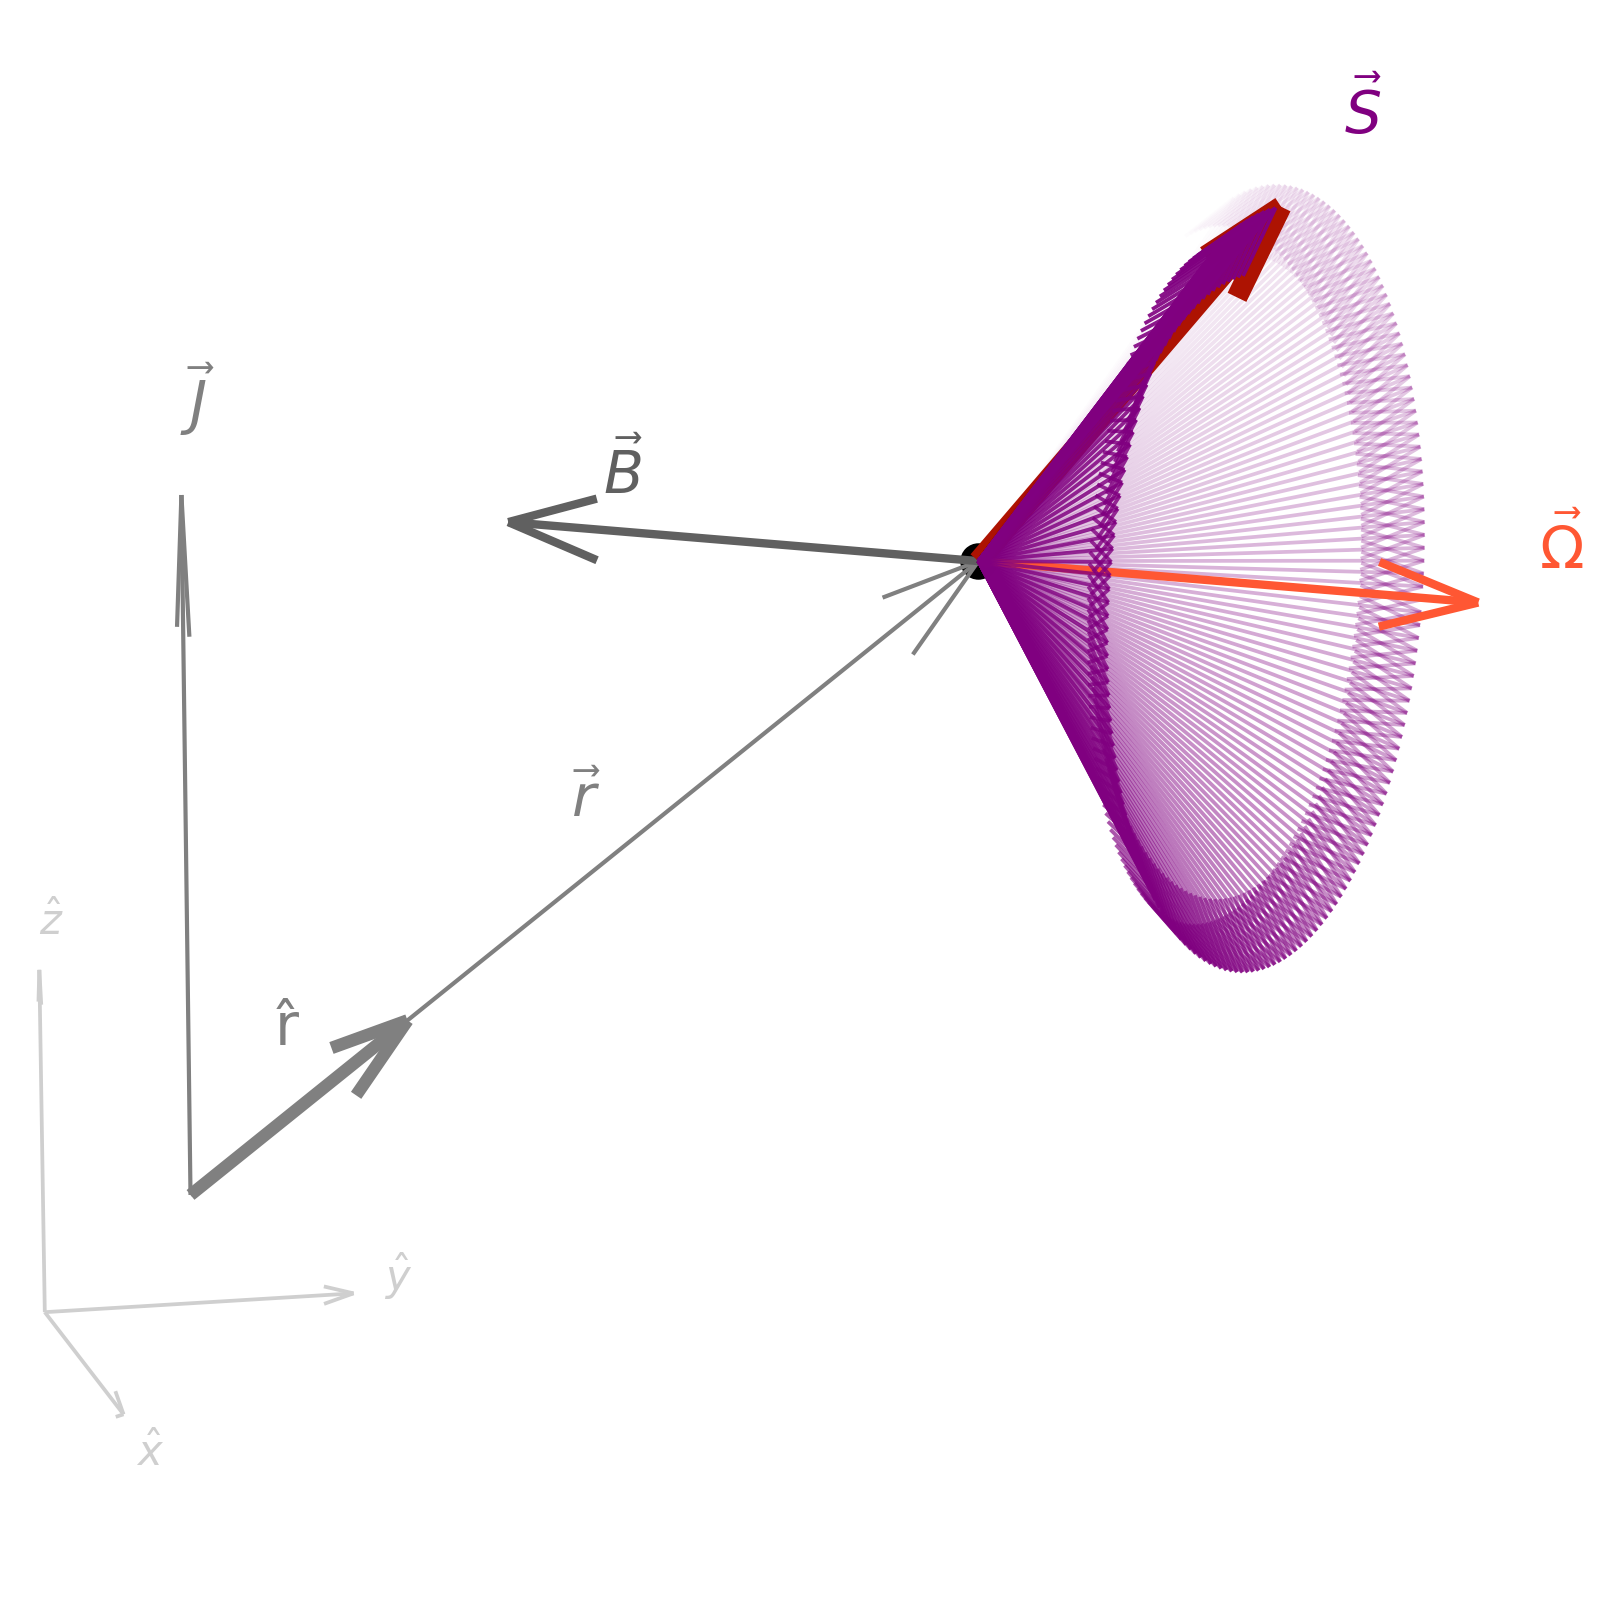
\includegraphics[width=\linewidth]{graphics/precesión_espín.png}

\vspace{0.2cm}
{\scriptsize Precesión del espín inducida por el campo gravitomagnético.}
\end{column}

\end{columns}

\end{frame}

%%%%%%%%%%%%%%%%%%%%%%%%%%%%%%%%%%%%%%%%%%%%%%%%%%%%%

\begin{frame}
\frametitle{Efecto de reloj gravitomagnético}

Para órbitas ecuatoriales ($\theta=\pi/2$), con la ecuación geodésica y la métrica de Kerr se tiene que:

\begin{equation}
g_{tt,r}\left(\frac{dt}{d\phi}\right)^2
+2 g_{t\phi,r}\frac{dt}{d\phi}
+g_{\phi\phi,r}=0
\end{equation}

entonces

\begin{equation}
\frac{dt}{d\phi}=\frac{a}{c}\pm \sqrt{\frac{r^3}{G_N M}}=\frac{a}{c}\pm \omega^{-1}
\end{equation}

donde $\omega=\sqrt{\frac{G_N M}{r^3}}$. Integrando

\begin{equation}
T_{\pm}=\frac{2\pi}{\omega}\pm \frac{2\pi a}{c}
\end{equation}

restando ahora $T_+-T_-$ se tiene el efecto de reloj gravitomagnético

\begin{equation}
T_+ - T_- = \frac{4\pi a}{c}
\end{equation}

\end{frame}


%%%%%%%%%%%%%%%%%%%%%%%%%%%%%%%%%%%%%%%%%%%%%%%%%%%%%%%

\begin{frame}
\frametitle{Efecto de reloj gravitomagnético para partículas con espín (MPD)}

\begin{columns}[t]

%----------------- COLUMNA 1 -----------------
\begin{column}{0.60\textwidth}
Las ecuaciones de movimiento sobre el plano ecuatorial MPD para la métrica de Kerr, fueron desarrolladas por (\cite{Saijo1998}). Luego (\cite{Jefremov2015}) determinó los parámetros para encontrar órbitas circulares estables. Velocidad angular

\begin{equation}
\Omega_s = \Omega_0 + s\,\Omega_1
\end{equation}

\begin{equation}
\frac{dt}{d\phi} \approx \frac{1}{\Omega_0} - s\frac{\Omega_1}{\Omega_0^2}
\end{equation}

\textbf{Tiempos orbitales}

\begin{align}
T_{\mp}=\mp 2\pi\left[\frac{a}{c}\mp \frac{1}{\sqrt{G_NM}\,u_0^{3/2}}-\,\frac{9s}{2\,c^2}\mp \frac{9a\sqrt{u_0}s}{2c\sqrt{G_NM}}\right]
\end{align}

\end{column}

%----------------- COLUMNA 2 -----------------
\begin{column}{0.35\textwidth}

restando los dos tiempos se tiene el efecto de reloj GEM para partículas con espín

\begin{equation}
T_+ - T_- = \frac{4\pi a}{c} - \frac{18\pi s}{c^2}
\end{equation}

\textbf{Caso especial}

\begin{itemize}
\item Co-rotante ($s>0$) + contra-rotante ($s<0$):
\end{itemize}

\begin{equation}
T_+ - T_- = \frac{4\pi a}{c}
\end{equation}


\end{column}

\end{columns}

\end{frame}

%%%%%%%%%%%%%%%%%%%%%%%%%%%%%%%%%%%%%%%%%%%%%%%%%%%%%
%%%%%%%%%%%%%%%%%%%%%%%%%%%%%%%%%%%%%%%%%%%%%%%%%%%%%
%%%%%%%%%%%%%%%%%%%%%%%%%%%%%%%%%%%%%%%%%%%%%%%%%%%%%

\section{Tensores de marea para la métrica de Schwarzschild y Kerr}
\begin{frame}[fragile]
\frametitle{Tensor de marea gravitomagnético para Schwarzschild}

\textbf{Código en Mathematica:}
\begin{lstlisting}[basicstyle=\ttfamily\scriptsize]
(*Calculo del tensor de marea gravitomagnetico (0,2)*)
TensorGMDD=Simplify[PowerExpand[Table[1/(2c)*(Sum[gDD[[\[Alpha],\[Eta]]]*gDD[[\[Lambda],\[Kappa]]]*1/(Sqrt[-detg])*epsilon[[\[Gamma],\[Delta],\[Eta],\[Kappa]]]*RiemannDDDD[[\[Gamma],\[Delta],\[Beta],\[Sigma]]]*uU[[\[Lambda]]]*uU[[\[Sigma]]],{\[Eta],n},{\[Lambda],n},{\[Kappa],n},{\[Gamma],n},{\[Delta],n},{\[Sigma],n}]),{\[Alpha],n},{\[Beta],n}]]];
\end{lstlisting}
Para la métrica de Schwarzschild
\begin{align}
\mathbb{H}_{t\theta}&=\mathbb{H}_{\theta t}=-\frac{3 r_s sin \theta}{2r}u^r u^\phi \\
\mathbb{H}_{t\phi}&=\mathbb{H}_{\phi t}=\frac{3 r_s sin \theta}{2r}u^r u^\theta \\
\mathbb{H}_{r\theta}&=\mathbb{H}_{\theta r}=\frac{3 r_s sin \theta}{2r}u^t u^\phi \\
\mathbb{H}_{r \phi}&=\mathbb{H}_{\phi r}=-\frac{3 r_s sin \theta}{2r}u^t u^\theta \\
\mathbb{H}_{tt}&=\mathbb{H}_{tr}=\mathbb{H}_{rt}=\mathbb{H}_{rr}=\mathbb{H}_{\theta\theta}=\mathbb{H}_{\theta\phi}=\mathbb{H}_{\phi\theta}=\mathbb{H}_{\phi\phi}=0
\end{align}

Si se impone $u^{\phi}=u^{\theta}=0$, se encuentra que el tensor de marea GM se anulan ($\mathbb{H}_{\mu\nu}=0$)
\end{frame}



\begin{frame}
\frametitle{Tensor de marea gravitomagnético para Kerr}
\begin{columns}

%----------------- COLUMNA 1 -----------------
\begin{column}{0.48\textwidth}

\begin{align*}
\mathbb{H}_{tt}&=-\frac{3acr_su^ru^{\theta}}{r^3}\\
\mathbb{H}_{tr}&=-\frac{3ar_s(-cu^tu^{\theta}+au^{\theta}u^{\phi})}{2r^3}\\
\mathbb{H}_{t\theta}&=-\frac{3r_su^r(-acu^t+a^2u^{\phi}+r^2u^{\phi})}{2r^3}\\
\mathbb{H}_{t\phi}&=\frac{3(2a^2+r^2)r_s u^r u^{\theta}}{2r^3}\\
\mathbb{H}_{rr}&=0
\end{align*}

\end{column}

%----------------- COLUMNA 2 -----------------
\begin{column}{0.48\textwidth}

\begin{align*}
\mathbb{H}_{r\theta}&=-\frac{3r_s(-cu^t+au^{\phi})(-acu^t+a^2u^{\phi}+r^2u^{\phi})}{2cr^3}\\
\mathbb{H}_{r\phi}&=\frac{3(a^2+r^2)r_su^{\theta}(-cu^t+au^{\phi})}{2cr^3}\\
\mathbb{H}_{\theta\phi}&=\frac{3ar_s u^r(-acu^t+a^2u^{\phi}+r^2u^{\phi})}{2cr^3}\\
\mathbb{H}_{\phi\phi}&=-\frac{3a(a^2+r^2)r_s u^r u^{\theta}}{cr^3}
\end{align*}

\end{column}

\end{columns}

donde $r_s=2G_N M/c^2$. Imponiendo que el observador se mueva sobre el plano ecuatorial, es decir, $u^{\theta}=0$, los términos $\mathbb{H}_{tt}=\mathbb{H}_{tr}=\mathbb{H}_{rt}=\mathbb{H}_{t\phi}=\mathbb{H}_{\phi t}=\mathbb{H}_{\phi r}=\mathbb{H}_{r \phi}=\mathbb{H}_{\phi\phi}$ se anulan. Por otro lado los términos $\mathbb{H}_{t\theta}$, $\mathbb{H}_{r\theta}$ y $\mathbb{H}_{\theta\phi}$ se anulan haciendo $-acu^t+a^2u^{\phi}+r^2u^{\phi}=0$
\begin{equation}\label{CondicionHnulaKerr}
\omega=\frac{d\phi}{dt}=\frac{u^{\phi}}{u^{t}}=\frac{ac}{a^2+r^2}
\end{equation}

\end{frame}

%%%%%%%%%%%%%%%%%%%%%%%%%%%%%%%%%%%%%%%%%%%%%%%%%%%%%%

\begin{frame}{Conclusiones}

\begin{itemize}

\item A lo largo del presente trabajo se presentaron de forma detallada analogías que facilitan la caracterización e interpretación del movimiento de una partícula con espín (momento angular de rotación) en un espacio-tiempo, a través de las ecuaciones de Mathisson-Papapetrou-Dixon.

\item Cuando se realiza la aproximación de campo y espín débil en las ecuaciones de MPD, se encuentra que el espín es análogo al momento dipolar magnético en el electromagnetismo, y que la fuerza de interacción entre un objeto de Kerr y una partícula con espín es análoga a la fuerza entre dos dipolos magnéticos.

\item Esto sugiere que existe una conexión con el gravitoelectromagnetismo desarrollado a partir de la aproximación de campo débil, en el que la métrica se describe como la métrica de Minkowski más una pequeña perturbación.

\item El espín de un objeto masivo de Kerr genera un campo gravitomagnético, el cual interactúa con el espacio-tiempo a su alrededor, generando el conocido efecto de frame-dragging.

\item La fuerza sobre una partícula sin espín está dada por $\mathbf{F}=m(\mathbf{E}+2\mathbf{v}\times\mathbf{B})$, mientras que para una partícula con espín es $\mathbf{F}_{GEM}=-\nabla U$, con $U=-\mathbf{S} \cdot \mathbf{B}_{GEM}$.

\item Otro fenómeno estudiado es el efecto de reloj gravitomagnético, cuyo desfase para partículas sin espín es $4\pi a/c$, y al incluir espín aparece un término adicional proporcional a $18\pi s/c^2$.

\end{itemize}

\end{frame}


%%%%%%%%%%%%%%%%%%%%%%%%%%%%%%%%%%%%%%%%%%%%%%%%%%%%%%%%%%%
\begin{frame}{Trabajo futuro}

\begin{itemize}

\item Las definiciones de los potenciales presentan ciertos grados de libertad que pueden ser tratados al considerar que la carga gravitomagnética sea el doble de la carga gravitoeléctrica, siendo este un aspecto en el que se puede profundizar.

\item Resulta pertinente profundizar en otro tipo de fuentes GEM y su interacción con partículas con espín.

\item Sería interesante profundizar en el papel de las condiciones suplementarias de espín en el efecto de reloj gravitomagnético.

\item También es importante analizar con mayor detalle la interpretación del término adicional asociado al espín en dicho efecto.

\item Otro aspecto que merece atención es investigar el efecto de reloj cuando se consideran órbitas no circulares.

\item Es importante seguir profundizando en las propiedades de simetría y de torsión del operador $\tilde{\nabla}$.

\item A la luz del formalismo Quasi-Maxwell, quedan abiertos problemas relacionados con el efecto de Lense-Thirring, el efecto de reloj gravitomagnético y otras aplicaciones astrofísicas o cosmológicas.

\item Aún queda por profundizar acerca de la interpretación física de las fuerzas inerciales en este formalismo.

\item Es importante revisar cómo se pueden encontrar o relacionar las analogías con otras condiciones suplementarias de espín.

\item Se debe trabajar en el tipo de órbitas que se mueven con velocidad angular $d\phi/dt=ac/(a^2+r^2)$ y bajo qué condiciones.

\item También queda por investigar aplicaciones astrofísicas o cosmológicas de estas analogías y la conexión entre ellas.

\item Resulta relevante investigar las propiedades de la estructura tipo agujero de gusano que emerge en la métrica de Kerr en el límite de masa cero, desde el punto de vista geométrico y topológico.

\end{itemize}

\end{frame}



% Comentar desde este punto hasta "\end{frame}" para no mostrar referencias. Esto se debe hacer sólo si NUNCA se usó el comando \cite en las diapositivas.
\section{Referencias}
\begin{frame}[allowframebreaks]
\frametitle{Referencias}
\scriptsize
%\bibliographystyle{amsalpha} %Estilo bibliografía.
%{\scriptsize \justifying
%\bibliography{references}
\printbibliography
\end{frame}

\end{document}
%%%%%%%%%%%%%%%%%%%%%%%%%%%%%%%%%%%%%%%%%%%%%%%%%%
%%%%%%%%%%%%%%%%%%%%%%%%%%%%%%%%%%%%%%%%%%%%%%%%%%
%%%%%%%%%%%%%%%%%%%%%%%%%%%%%%%%%%%%%%%%%%%%%%%%%%